%%%%%%%%%%%%%%%%%%%%%%%%%%%%%%%%%%%%%%%%%%%%%%%%%%%%%%%%%%%%%%%%%%%%%%%%%%%
%%%%% sub sequence
%%%%%%%%%%%%%%%%%%%%%%%%%%%%%%%%%%%%%%%%%%%%%%%%%%%%%%%%%%%%%%%%%%%%%%%%%%%
\documentclass[../../../main.tex]{subfiles}
\begin{document}
\section{Subsequence (Medium or Hard)}
The difference of the subsequence type of questions with the subarray is that we do not need the elements to be consecutive. Because of this relaxation, the brute force solution of this type of question is exponential$O(2^n)$, because for each element, we have two options: chosen or not chosen. This type of questions would usually be used as a follow-up question to the subarray due to its further difficulty because of nonconsecutive. This type of problems are a typical dynamic programming. Here we should a list of all related subsequence problems shown on LeetCode in Fig.~\ref{fig:subsequence_problems}

A subsequence of a string is a new string which is formed from the original string by deleting some (can be none) of the characters without disturbing the relative positions of the remaining characters. (ie, "ACE" is a subsequence of "ABCDE" while "AEC" is not). For the subsequence problems, commonly we will see increasing subsequence, count the distinct subsequence. And they are usually solved with single sequence type of dynamic programming. 
\begin{figure}[h]
    \centering
    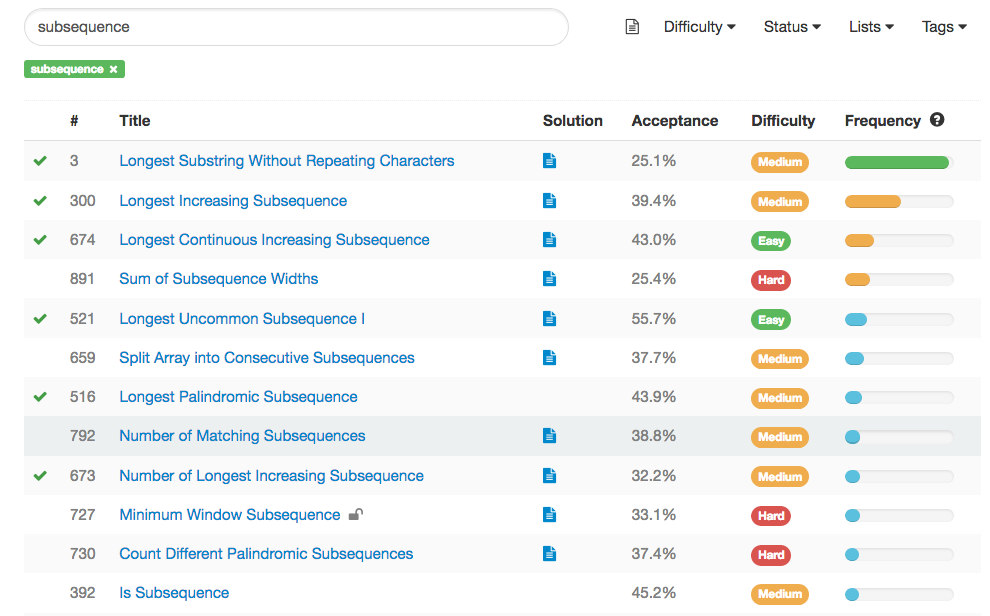
\includegraphics[width=0.8\columnwidth]{fig/subsequence_1.png}
    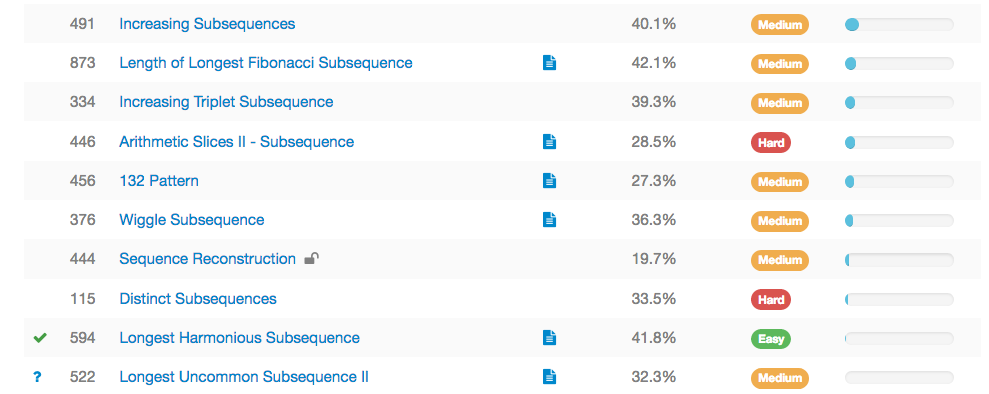
\includegraphics[width=0.8\columnwidth]{fig/subsequence_2.png}
    \caption{Subsequence Problems Listed on LeetCode}
    \label{fig:subsequence_problems}
\end{figure}
940. Distinct Subsequences II (hard)

Given a string S, count the number of distinct, non-empty subsequences of S . Since the result may be large, return the answer modulo $10^9 + 7$.
\begin{lstlisting}
Example 1:

Input: "abc"
Output: 7
Explanation: The 7 distinct subsequences are "a", "b", "c", "ab", "ac", "bc", and "abc".

Example 2:

Input: "aba"
Output: 6
Explanation: The 6 distinct subsequences are "a", "b", "ab", "ba", "aa" and "aba".

Example 3:

Input: "aaa"
Output: 3
Explanation: The 3 distinct subsequences are "a", "aa" and "aaa".
\end{lstlisting}
\textbf{Sequence type dynamic programming}. The naive solution for subsequence is using DFS to generate all of the subsequence recursively and we also need to check the repetition. The possible number of subsequence is $2^n-1$. Let's try forward induction method. 
\begin{lstlisting}
# define the result for each state: number of subsequence ends with each state
state:  a   b  c
ans  :  1   2  4 
a: a; dp[0] = 1
b: b, ab; = dp[0]+1 if this is 'a', length 1 is the same as dp[0], only length 2 is possible
c: c, ac, bc, abc; = dp[0]+dp[1]+1, if it is 'a', aa, ba, aba,  = dp[1]+1
d: d, ad, bd, abd, cd, acd, bcd, abcd = dp[0]+dp[1]+dp[2]+1
\end{lstlisting}
Thus the recurrence function can be Eq.~\ref{eq:distinct_subsequence}.
\begin{equation}
\label{eq:distinct_subsequence}
    dp[i] = \sum_{j<i}(dp[j]) +1, S[j] != S[i]
\end{equation}
Thus, we have $O(n^2)$ time complexity, and the following code:
\begin{lstlisting}[language=Python]
def distinctSubseqII(self, S):
    """
    :type S: str
    :rtype: int
    """
    MOD = 10**9+7
    dp = [1]*len(S) #means for that length it has at least one count
    for i, c in enumerate(S):
        for j in range(i):
            if c == S[j]:
                continue
            else:
                dp[i] += dp[j]
                dp[i] %= MOD
    return sum(dp) % MOD
\end{lstlisting}
However, we still get LTE. How to improve it further. If we use a counter indexed by all of the 26 letters, and a prefix sum. The inner for loop can be replaced by dp[i] = 1+ (prefix sum - sum of all S[i]).Thus we can lower the complexity further to $O(n)$.
\begin{lstlisting}[language=Python]
def distinctSubseqII(self, S):
    MOD = 10**9+7
    dp = [1]*len(S) #means for that length it has at least one count
    sum_tracker = [0]*26
    total = 0
    for i, c in enumerate(S):
        index = ord(c) - ord('a')
        dp[i] += total-sum_tracker[index]
        total += dp[i]
        sum_tracker[index] += dp[i]
    return sum(dp) % MOD
\end{lstlisting}

%%%%%%%%%%%%%%%%%%%%%%%%%%%%%%%%%%%%%%%%%%%%%%%%%%%%%%%%%%%%%%%%%%%%%%%%%%%
%%%%% Sum
%%%%%%%%%%%%%%%%%%%%%%%%%%%%%%%%%%%%%%%%%%%%%%%%%%%%%%%%%%%%%%%%%%%%%%%%%%%
% \subsection{Sum}
% In this section, to get sum we can choose to use hashmap to save the original list so that for the last element, we only check the hashmap, we can lower the complexity by one power of n. However, a better solution is to use two pointers or three pointers. for three pointers, the first one is to make sure the starting point. Also, we can think about divide and conquer.
% \begin{lstlisting}
% [-4,-1,-1,0,1,2]
% i, l-> ``````<-r
% \end{lstlisting}

% \begin{enumerate}
%     \item 
%%%%%%%%%%%%%%%%%%%%%%%%%%%%%%%%%%%%%%%%%%%%%%%%%%%%%%%%%%%%%%%%%%%%%%%%%%%
%%%%% Others
%%%%%%%%%%%%%%%%%%%%%%%%%%%%%%%%%%%%%%%%%%%%%%%%%%%%%%%%%%%%%%%%%%%%%%%%%%%
\subsection{Others}
For example, the following question would be used as follow up for question \textit{Longest Continuous Increasing Subsequence}

300. Longest Increasing Subsequence


673. Number of Longest Increasing Subsequence

Given an unsorted array of integers, find the number of longest increasing subsequence.
\begin{lstlisting}
Example 1:

Input: [1,3,5,4,7]
Output: 2
Explanation: The two longest increasing subsequence are [1, 3, 4, 7] and [1, 3, 5, 7].

Example 2:
Input: [2,2,2,2,2]
Output: 5
Explanation: The length of longest continuous increasing subsequence is 1, and there are 5 subsequences' length is 1, so output 5.
\textit{Note: Length of the given array will be not exceed 2000 and the answer is guaranteed to be fit in 32-bit signed int.}
\end{lstlisting}

Solution: Another different problem, to count the number of the max subsequence. Typical dp:

state: f[i]
\begin{lstlisting}[language = Python]
from sys import maxsize
class Solution:
    def findNumberOfLIS(self, nums):
        """
        :type nums: List[int]
        :rtype: int
        """
        max_count = 0
        if not nums:
            return 0
        memo =[None for _ in range(len(nums))]
        rlst=[]
        def recursive(idx,tail,res):
            if idx==len(nums):
                rlst.append(res)
                return 0
            if memo[idx]==None:
                length = 0
                if nums[idx]>tail:
                    addLen = 1+recursive(idx+1, nums[idx],res+[nums[idx]])
                    notAddLen = recursive(idx+1, tail,res)
                    return max(addLen,notAddLen)
                else:
                    return recursive(idx+1, tail,res)
        
        
        ans=recursive(0,-maxsize,[])
        count=0
        for lst in rlst:
            if len(lst)==ans:
                count+=1
                
        return count
\end{lstlisting}

Using dynamic programming, the difference is we add a count array.
\begin{lstlisting}[language = Python]
from sys import maxsize
class Solution:
    def findNumberOfLIS(self, nums):
        N = len(nums)
        if N <= 1: return N
        lengths = [0] * N #lengths[i] = longest ending in nums[i]
        counts = [1] * N #count[i] = number of longest ending in nums[i]

    for idx, num in enumerate(nums): #i
            for i in range(idx): #j
                if nums[i] < nums[idx]: #bigger 
                    if lengths[i] >= lengths[idx]:
                        lengths[idx] = 1 + lengths[i] #set the biggest length
                        counts[idx] = counts[i] #change the count
                    elif lengths[i] + 1 == lengths[idx]: #if it is a tie
                        counts[idx] += counts[i] #increase the current count by count[i]

longest = max(lengths)
        print(counts)
        print(lengths)
        return sum(c for i, c in enumerate(counts) if lengths[i] == longest)
\end{lstlisting}

128. Longest Consecutive Sequence
\begin{lstlisting}
Given an unsorted array of integers, find the length of the longest consecutive elements sequence.

For example,
 Given [100, 4, 200, 1, 3, 2],
 The longest consecutive elements sequence is [1, 2, 3, 4]. Return its length: 4.
 
 Your algorithm should run in O(n) complexity.
 \end{lstlisting}

Solution: Not thinking about the O(n) complexity, we can use sorting to get [1,2,3,4,100,200], and then use two pointers to get [1,2,3,4].

How about O(n)? We can pop out a number in the list, example, 4 , then we use while first-1 to get any number that is on the left side of 4, here it is 3, 2, 1, and use another to find all the bigger one and remove these numbers from the nums array.
\begin{lstlisting}[language =Python]
def longestConsecutive(self, nums):
        nums = set(nums)
        maxlen = 0
        while nums:
            first = last = nums.pop()
            while first - 1 in nums: #keep finding the smaller one
                first -= 1
                nums.remove(first)
            while last + 1 in nums: #keep finding the larger one
                last += 1
                nums.remove(last)
            maxlen = max(maxlen, last - first + 1)
        return maxlen
\end{lstlisting}
\end{document}